\documentclass[11pt]{article}
\usepackage[includeheadfoot, top=1.0in, bottom=1.0in, hmargin=1.0in]{geometry}
\usepackage[utf8]{inputenc}
\usepackage{fancyhdr}
\usepackage{url}
\pagestyle{fancy}
\usepackage{setspace}
\usepackage{tabularx}
\usepackage{graphicx}
\usepackage{caption}
\usepackage{subcaption}
\usepackage{hyperref}
\usepackage{multicol}

\usepackage{hyperref}
\hypersetup{
    colorlinks=true,
    linkcolor=blue,
    filecolor=magenta,      
    urlcolor=blue,
}


\lhead{Astronomy Lab II}
\rhead{Fall 2024}
\lfoot{Porter}
\rfoot{Wed 6-9pm}
\cfoot{\thepage}

\begin{document}

\begin{center}
\huge{Lab 5: Galaxy Classification}\\ \medskip \Large{October 9, 2024}
\end{center}

%%%%%%%%%%%%%%%%%%%%%%% INTRO %%%%%%%%%%%%%%%%%%%%%%%
\section{Introduction: In a Galaxy Far, Far Away}
In the early 20th century, there was a strong tension amongst astronomers regarding the nature of some faint, fuzzy objects that could barely be resolved with a telescope. Some astronomers believed that these ``nebulae" were clusters of stars in our own Milky Way, while others believed that they were their own distant, independent islands of stars. This disagreement has since been deemed \textit{The Great Debate}. It wasn't until 1924 -- when Edwin Hubble measured the distance to one of these nebulae -- that astronomers were able to settle the debate: Hubble found the Andromeda ``nebula'' to be over \emph{2 million light years} away, confirming that this was indeed a \textbf{galaxy} far, far away (cue the \href{https://www.youtube.com/watch?v=MNMSAIG0dfQ}{Star Wars music}).


\medskip
Since Hubble's discovery, astronomers have studied galaxies with great interest. Galaxies come in all shapes, sizes, colors, and luminosities.  Each of these properties can tell us something unique about a galaxy: we can learn about the stars and gas within the galaxy, or the amount of dark matter permeating the galaxy; we can learn about the age of the galaxy and its evolutionary history; and we can learn about the galaxy's surrounding environment and the interactions that this environment induces. The first step in understanding a galaxy is to determine what \emph{type} of galaxy it is -- and we can do this by just looking at it!  Today, we'll think about the \textit{morphology} (or shape and structure) of galaxies and what we can learn from that. The goals of today's lab are for you to get a sense of the diversity of galaxies in the Universe, to create and test a galaxy classification system of your own, and to learn what the morphology of a galaxy can tell us about its evolutionary state.

\medskip
\textbf{Answer the following in your lab write-up}:

\begin{enumerate}
\setcounter{enumi}{0}

    \item Before beginning this lab, after listening to the short intro, what do you think are the most important things astronomer should consider when determining a galaxy's shape (a.k.a. morphology)? Pick three things and justify your answer. 
    
\end{enumerate}
\medskip


%%%%%%%%%%%%%%%%%%%%%%% HUBBLE TUNING FORK %%%%%%%%%%%%%%%%%%%%%%%
\section{The Hubble Tuning Fork}

\begin{figure} [h!]
    \centering
    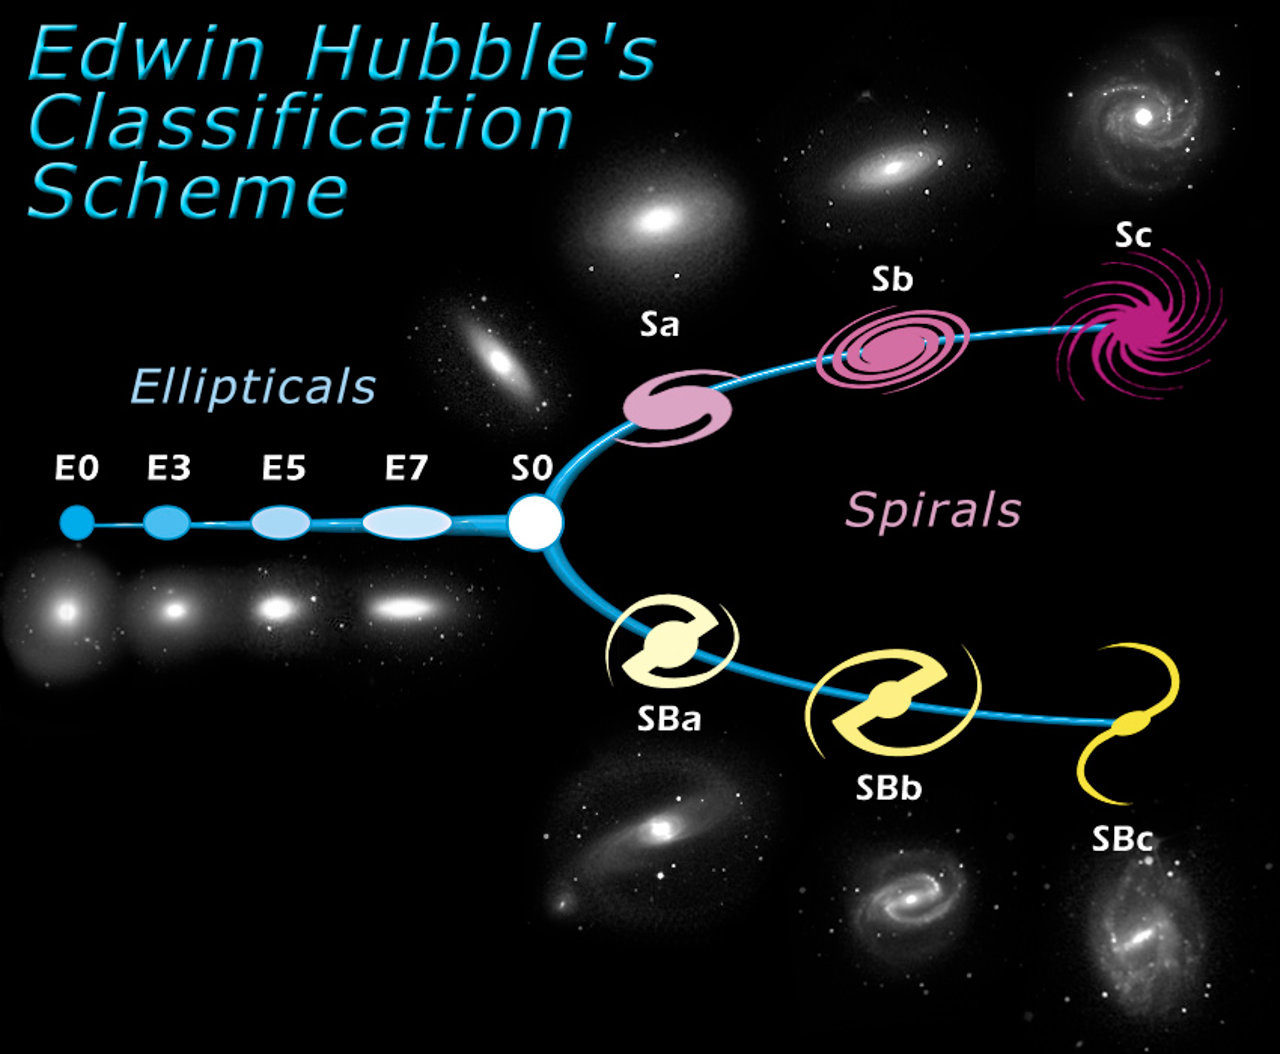
\includegraphics[width=0.7\textwidth]{Images/image.png}
    \caption{The Hubble tuning fork. Credit: NASA/ESA}
    \label{fig:Hubble}
\end{figure}

\noindent
Figure \ref{fig:Hubble} shows a simplified schematic of the galaxy classification system that we typically use in modern astronomy -- this diagram is known as the \textit{``Hubble tuning fork''} (or the ``Hubble classification system,'' or the ``Hubble sequence''). The Hubble sequence is a \emph{morphological} galaxy classification scheme introduced by Edwin Hubble in 1936 (the nickname of ``tuning fork'' comes from the shape in which this system is traditionally represented). Hubble's scheme divides galaxies into \emph{three} broad classes based on their visual appearance. \textbf{Answer the following in your lab write-up}:
\medskip
\begin{enumerate}
\setcounter{enumi}{1}
    \item There are three primary branches depicted on the tuning fork. 
    \begin{enumerate}
        \item What features distinguish each of the three branches from one another? (that is, how are the galaxies along one branch unique from the galaxies along the other two branches?)
        
        \item How do the galaxies \emph{within} each branch vary?
    \end{enumerate}
    
    \item Is there anything about this classification branch that doesn't make sense to you? Do you think astronomers today still use this method?
    
\end{enumerate}
\medskip

\noindent
You probably noted some of the following features in your description of the Hubble tuning fork; here are the formal names and descriptions for the galaxy types represented in Hubble's classification system:

\begin{itemize}
    \item \underline{Elliptical galaxies} (to the left of the tuning fork) appear as smooth, featureless ellipses in images. They are denoted by the letter `E,' followed by an integer `n' representing their degree of ``ellipticity'' (with $n=0$ being a spherical galaxy and $n=7$ being a very stretched-out ellipsoidal galaxy).
    
    \item \underline{Spiral galaxies} (to the right of the tuning fork) consist of a flattened ``disk'' with stars forming a spiral structure, along with a central concentration of stars known as the ``bulge,'' which is similar in appearance to an elliptical galaxy. Roughly half of all spirals are also observed to have a bar-like structure extending from the central bulge -- these ``barred spirals'' (on the bottom right of the tuning fork) are given the label `SB.' \emph{Unbarred} spiral galaxies (on the upper right of the tuning fork) are labeled with the letter `S.' Our own Milky Way is a barred spiral.
    
    \item \underline{Lenticular galaxies} (at the center of the tuning fork) also consist of a bright central bulge surrounded by an extended disk-like structure -- but, unlike spiral galaxies, the disks of lenticular galaxies have no visible spiral structures and are not actively forming stars in any significant quantity. Lenticular galaxies are labeled `S0.'
    
    \item \underline{Irregular Galaxies} do not fit into the Hubble sequence, because they have no regular structure (neither disk-like nor ellipsoidal). Irregular galaxies are labeled `Irr.'
\end{itemize}


\noindent
\textbf{Here's a fun fact:} The Hubble tuning fork is drawn the way it is because astronomers originally thought that galaxies evolved from \emph{left} to \emph{right} along the diagram -- they thought that galaxies were formed as \textit{elliptical} galaxies and then evolved into \textit{spiral} galaxies, finally morphing into \textit{irregular} galaxies. We now think that galaxies do \emph{the exact opposite}, and are born as irregular galaxies, form spirals through interactions with other galaxies, and then finally end up as elliptical, featureless galaxies.
\medskip

\subsection{The JWST Deep Field}
%Introduce the Deep Field

Navigate to \url{https://www.nasa.gov/wp-content/uploads/2023/03/main_image_deep_field_smacs0723-5mb.jpg}. \\\textbf{\textit{Whoa}}, right? This image is known as the \textit{JWST Deep Field}. The snapshot includes a myriad galaxies of various ages, sizes, shapes, and colors. The smallest, reddest galaxies may be among the most distant and oldest known, existing when the Universe was just 300 million years old (so, more tha 14 billion years ago) - and we can see them!

\medskip \noindent
\textbf{Complete the following in your lab write-up}:
\begin{enumerate}
\setcounter{enumi}{3}
    \item With the exception of a few stars in this image, every object you see is a galaxy. Try to identify the stars. How many are there, and how did you identify them? Circle them in a bright color, if possible.
    
    \item Deep Field images, such as the one here or the Hubble Deep Field, are known for the amount of galaxies they are able to capture in such a "deep" exposure - this isn't much different from taking a photo with a long exposure time. 
    \begin{enumerate}
        \item Estimate the total number of galaxies you see in the JWST Deep Field.  Remember, this is an estimate - you don't need to count each one. 

        \item Note that this image covers a VERY small portion of the sky - the same space as if you held up a grain of sand as far as you could. What does this tell you about the number of galaxies in the Universe? 
        
    \end{enumerate}
    
    \item About what fraction of the Field are spiral galaxies? What fraction are elliptical galaxies?

    \item Are there any especially odd galaxies in this image? What makes them odd, and why do you think they look this way?

\end{enumerate}

\medskip


%%%%%%%%%%%%%%%%%%%%%%% GALAXY ZOO %%%%%%%%%%%%%%%%%%%%%%%
\section{Galaxy Zoo}

Navigate to \url{https://www.zooniverse.org/projects/zookeeper/galaxy-zoo/}. ``Galaxy Zoo'' is a citizen science project that invites amateur astronomers to help categorize large data sets of galaxy images. Once you're on the Galaxy Zoo main page, click ``Get Started" and read through the instructions; if you need some help, you can click on ``Need some help with this task?" or pull out the ``Field Guide" to the right of the screen. For the first galaxy you look at, I highly recommend reading through some of the examples under ``Need some help with this task?" 

\medskip \noindent
Classify about 15 galaxies on Galaxy Zoo. \textbf{Complete the following in your lab write-up}:
\begin{enumerate}
\setcounter{enumi}{7}

    \item Take a screenshot and log which galaxies you classify. You don't have to note all of the decisions you made.
    
    \item Reflect on anything unusual you saw in the galaxies on Galaxy Zoo. Did you notice any unique features? What made it easier or more difficult for you to catalog galaxies?

    \item What do you think about these methods of using citizen science projects like Galaxy Zoo? What are some potential pros and cons? Justify your thoughts.
\end{enumerate}

%%%%%%%%%%%%%%%%%%%%%%% CHANGING A GALAXY'S SHAPE %%%%%%%%%%%%%%%%%%%%%%%
\section{What Changes a Galaxy's Shape?}

Now that we've established how galaxies have different shapes and sizes, you might be wondering what can actually cause a galaxy's shape to change. However, this is a field in galaxies that we still don't know a lot about: we have some general intuition and a few theories, but this is still an active field of study. For example, bars in galaxies are thought to possibly be connected to Active Galactic Nuclei (AGN). Galaxies that collide together can also experience a drastic change in their shape.

Navigate to this video \url{https://www.youtube.com/watch?v=QcDtJ_-jdMw}, a simulation of two galaxies merging together. Mergers are thought to be one of the primary reasons for the change in galaxy shapes, and is how many of the most massive galaxies grow. \textbf{Record the following in your lab write-up. Please be detailed in your answers.}
\begin{enumerate}
\setcounter{enumi}{10}
    
    \item What do you notice about the shapes of the galaxies before the collision?
    
    \item What happens to each galaxy during the collision?
    
    \item How is the final shape different as both galaxies coalesce into one?

    \item You may have already learned (either in this lab or lecture) that the Universe is expanding over time. If you haven't heard of this before, we'll discuss it more later in both lab and lecture.
    \begin{enumerate}
        \item Using this fact, do you think galaxies would be more likely to merge early in the Universe while it was young, or at later times such as now? Justify your answer. 


        \item How do you think galaxy environment can affect the morphology of a galaxy? Explain your answer. 
        
    \end{enumerate}
    
\end{enumerate}

\medskip


%%%%%%%%%%%%%%%%%%%%%%% CONCLUSIONS %%%%%%%%%%%%%%%%%%%%%%%
\section{Wrapping Things Up}
\textbf{Answer the following questions in your lab write-up}:
\begin{enumerate}
\setcounter{enumi}{14}
    
    \item List some factors that might make classifying galaxies a difficult task, and why they make it difficult.
    
    \item Describe the Hubble tuning fork and how it functions as a galaxy classification system.
    
    \item Considering the wide variety of galaxies that you saw in the JWST Deep Field. Beyond morphology (i.e., shape) what are some other features that we could use to classify galaxies?
    
\end{enumerate}


There are many citizen science research projects like Galaxy Zoo that \emph{YOU} can participate in. Check out some of them here: \url{https://www.zooniverse.org/projects?discipline=astronomy&page=1&status=live}


\end{document}
